% Week 1 Session B — AI Mental Models (CoT vs direct prompting)
% All lab reports in this series include an abstract (see Session A/B .tex).
%
% Build: pdflatex Week1_SessionB_Report.tex from Lab-reports/
% Same folder: week1_session_b_opencode.png, week1_session_b_opencode2.png,
%   week1_session_b_opencode3.png, prompt_log_week1_session_b.md (copy from week1_session_b/)
%
\documentclass[11pt,a4paper]{article}

\usepackage[margin=2.5cm]{geometry}
\usepackage{graphicx}
\usepackage{booktabs}
\usepackage{xurl}
\usepackage{hyperref}
\usepackage{parskip}
\usepackage{enumitem}
\usepackage{xcolor}
\usepackage{fvextra}
\usepackage[most]{tcolorbox}

\newcommand{\studentname}{Your Name}
\newcommand{\studentid}{Your Student ID}
\newcommand{\reportdate}{May 16, 2026}

\makeatletter
\g@addto@macro\UrlBreaks{\do\ }
\makeatother

\newcommand{\LabCodeRoot}{.}

\title{Lab Report: Week 1 Session B\\AI Mental Models --- Chain-of-Thought Practice}
\author{\studentname \quad (\studentid)}
\date{\reportdate}

\begin{document}
\maketitle

\begin{abstract}
This report documents Week~1 Session~B: comparing \textbf{chain-of-thought} and \textbf{direct} prompting with OpenCode Desktop on reservoir storage (500~ha, 15~m depth $\rightarrow$ 75~MCM) and SCS-CN runoff ($P=80$~mm, $\mathrm{CN}=85$ $\rightarrow$ $Q=43.6$~mm). Both runoff prompts agreed numerically; CoT required explicit verification ($Q \le P$). Evidence includes three OpenCode screenshots and the full \path{prompt_log.md} in Appendix~\ref{app:promptlog}.
\end{abstract}

\section{Introduction}
This session practiced \textbf{prompting strategy} for hydrology and water-resources calculations using OpenCode Desktop with OpenCode Zen. Two styles were compared: a \textbf{chain-of-thought (CoT)} prompt that requests numbered reasoning steps, and a \textbf{direct} one-line question. Exercises covered reservoir storage volume (unit conversion and magnitude check) and SCS-CN direct runoff for 80~mm rainfall with curve number 85.

\section{Objectives}
\begin{itemize}[noitemsep]
  \item Practice CoT prompting with explicit steps and verification.
  \item Compare direct vs.\ step-by-step AI responses on the same hydrologic problem.
  \item Document prompts, outputs, and verification in a prompt log.
  \item Reflect on when each prompting style is appropriate.
\end{itemize}

\section{Methods}
Work was carried out in \path{ai_water_lab/week1_session_b/} using OpenCode Desktop. No Python script was required for this lab; results are AI-generated calculations recorded in \path{prompt_log.md} and supported by OpenCode session screenshots (Figures~\ref{fig:reservoir}--\ref{fig:cot}).

\subsection{Exercise 1: Reservoir capacity (CoT)}
The lab prompt specified 500~ha surface area and 15~m average depth, with steps to convert hectares to square metres, compute volume, express result in million cubic metres (MCM), and comment on whether the value is reasonable for a medium-sized reservoir.

\subsection{Exercise 2: SCS-CN runoff (direct vs.\ CoT)}
The same rainfall depth ($P = 80$~mm) and curve number ($\mathrm{CN} = 85$) were used twice:
\begin{itemize}[noitemsep]
  \item \textbf{Direct:} \emph{Calculate the runoff for 80mm rainfall with CN=85}
  \item \textbf{CoT:} same problem with explicit steps for $S$, $I_a$, the SCS-CN formula, and verification $Q \le P$.
\end{itemize}
The standard SCS-CN relations used were $S = (25400/\mathrm{CN}) - 254$, $I_a = 0.2S$, and for $P > I_a$, $Q = (P-I_a)^2/(P-I_a+S)$.

\section{Results}

\subsection{Exercise 1: Reservoir storage}
The AI solution gave:
\begin{itemize}[noitemsep]
  \item Area: $500~\mathrm{ha} = 5{,}000{,}000~\mathrm{m}^2$
  \item Volume: $75{,}000{,}000~\mathrm{m}^3$
  \item Storage: \textbf{75~MCM}
\end{itemize}
Figure~\ref{fig:reservoir} shows the OpenCode conversation for this prompt.

\begin{figure}[htbp]
  \centering
  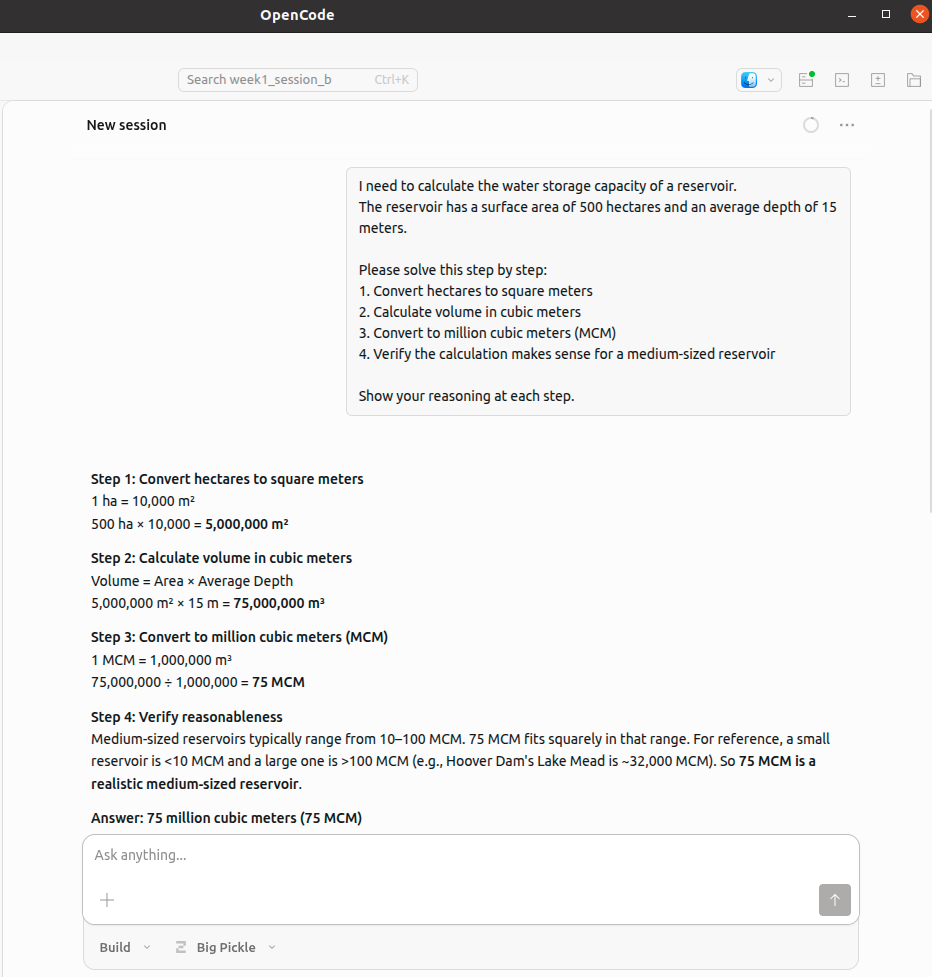
\includegraphics[width=0.95\textwidth]{week1_session_b_opencode.png}
  \caption{OpenCode session: chain-of-thought reservoir capacity calculation (Exercise~1).}
  \label{fig:reservoir}
\end{figure}

\subsection{Exercise 2: Direct SCS-CN prompt}
The direct prompt produced $S = 44.82$~mm, $I_a = 8.96$~mm, and runoff $Q = 43.6$~mm, with intermediate algebra shown. Figure~\ref{fig:direct} documents this exchange.

\begin{figure}[htbp]
  \centering
  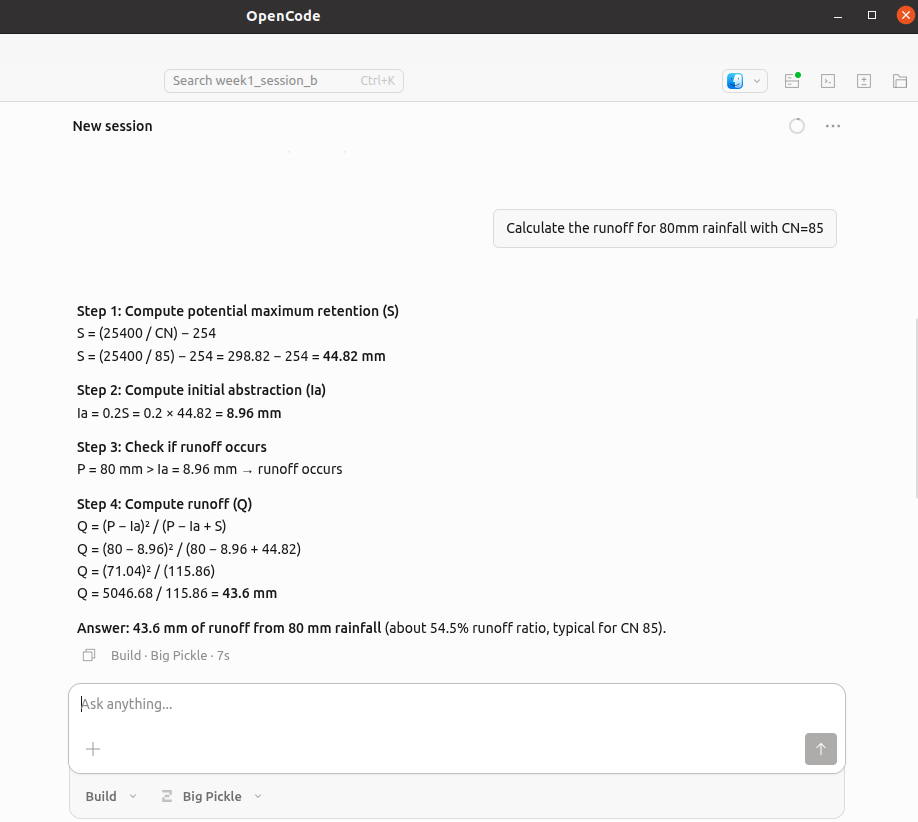
\includegraphics[width=0.95\textwidth]{week1_session_b_opencode2.png}
  \caption{OpenCode session: direct prompt for SCS-CN runoff ($P=80$~mm, $\mathrm{CN}=85$).}
  \label{fig:direct}
\end{figure}

\subsection{Exercise 2: CoT SCS-CN prompt}
The structured prompt yielded the same $Q = 43.6$~mm and explicitly verified $Q \le P$. Figure~\ref{fig:cot} shows this session.

\begin{figure}[htbp]
  \centering
  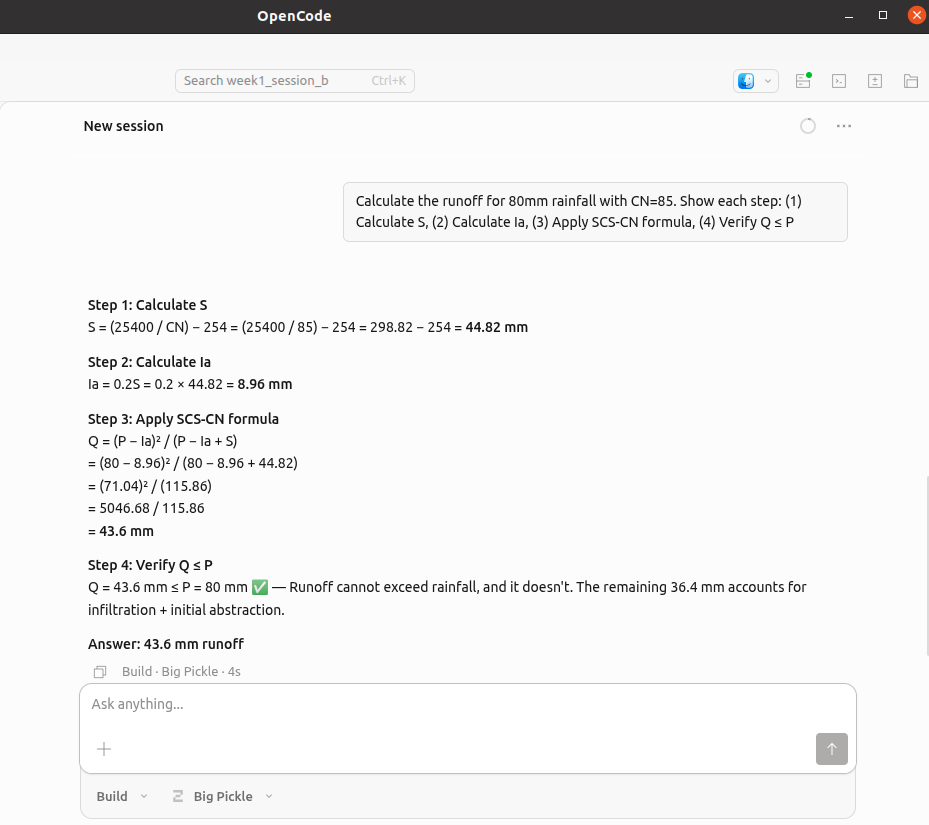
\includegraphics[width=0.95\textwidth]{week1_session_b_opencode3.png}
  \caption{OpenCode session: chain-of-thought SCS-CN calculation with $Q \le P$ verification.}
  \label{fig:cot}
\end{figure}

Table~\ref{tab:scscn} summarizes both runoff prompts.

\begin{table}[htbp]
  \centering
  \caption{Comparison of direct vs.\ CoT prompts for SCS-CN runoff ($P=80$~mm, $\mathrm{CN}=85$).}
  \label{tab:scscn}
  \begin{tabular}{@{}lll@{}}
    \toprule
    Item & Direct prompt & CoT prompt \\
    \midrule
    Final $Q$ & 43.6~mm & 43.6~mm \\
    Steps shown & Yes (unprompted) & Yes (requested) \\
    $Q \le P$ check & Implicit in narrative & Explicit step \\
    \bottomrule
  \end{tabular}
\end{table}

\section{Analysis and validation}

\textbf{Reservoir (Exercise~1):} Manual recomputation confirms 75~MCM. The CoT structure separated unit conversion, volume, and scaling, which reduces the risk of mixing hectares with square metres or forgetting the $10^6$ factor for MCM.

\textbf{SCS-CN (Exercise~2):} Independent check: $S = 25400/85 - 254 = 44.82$~mm; $I_a = 8.96$~mm; $P - I_a = 71.04$~mm; $Q = 71.04^2 / 115.86 \approx 43.6$~mm; $Q < P$. Both AI answers match this check.

\textbf{Direct vs.\ CoT:} The numeric answers agreed. The main difference is \emph{process control}: CoT prompts force verification steps that are easy to grade and to defend in a report. The direct prompt still produced detailed work here, but that behaviour is not guaranteed for every model or every problem.

\textbf{Limitations:} AI reasoning is not a substitute for design standards, antecedent moisture adjustments, or site data. Reservoir ``reasonableness'' ranges cited by the model are qualitative.

\section{Discussion}
\begin{enumerate}[noitemsep]
  \item CoT increased confidence because each step could be checked against textbook formulas; the direct answer was equally numeric but less structured.
  \item Step-by-step prompts suit multi-unit conversions, method-based hydrology (SCS-CN, routing), and any graded work requiring shown work.
  \item Even with ``show your work,'' the user must verify units, boundary conditions ($P < I_a$), and $Q \le P$.
  \item Next session: specify output format and verification checks in the prompt from the start (as in the CoT runoff prompt).
\end{enumerate}

\section{Problems encountered}
No calculation errors were found after manual verification. The main practical issue is documenting three separate OpenCode exchanges; screenshots were saved for each prompt.

\section{Lessons learned}
Structured prompts align AI output with engineering documentation habits. When direct and CoT answers match, CoT still adds audit value. Keeping a prompt log alongside screenshots makes report writing straightforward and satisfies the course submission requirements.

\section{Conclusion}
Week~1 Session~B objectives were met: CoT reservoir calculation (75~MCM), comparison of direct and CoT SCS-CN runoff (both 43.6~mm), and documentation in \path{prompt_log.md} with OpenCode evidence. Course submission: \path{prompt_log.md} and screenshots as specified in the lab guide.

\appendix

\section{Submitted prompt log: \path{prompt\_log.md}}
\label{app:promptlog}
\begin{tcolorbox}[
  enhanced,
  colback=gray!6,
  colframe=black!55,
  title={\path{prompt_log.md} \mdseries (full file)},
  fonttitle=\bfseries\ttfamily\footnotesize,
  arc=1.5mm,
  boxrule=0.7pt,
  breakable,
  width=\linewidth,
  before skip=0.8em,
  after skip=0.8em,
]
\VerbatimInput[
  fontsize=\footnotesize,
  breaklines=true,
  breakanywhere=true,
]{\LabCodeRoot/prompt_log_week1_session_b.md}
\end{tcolorbox}

\end{document}
